\documentclass[conference]{IEEEtran}
\IEEEoverridecommandlockouts
\usepackage[T1]{fontenc}
\usepackage[utf8]{inputenc}
\usepackage{cite,amsmath,amssymb,graphicx,booktabs,array,tabularx}
\usepackage{algorithm,algorithmic}
\usepackage{tikz,pgfplots}
\usepackage[hyphens]{url}
\usepackage{xurl}
\usepackage[hidelinks]{hyperref}
\usepackage{microtype}
\usetikzlibrary{arrows.meta,positioning,calc}
\pgfplotsset{compat=1.17}
\definecolor{inkblue}{RGB}{42,97,130}
\definecolor{mutedgreen}{RGB}{71,123,103}
\definecolor{mutedamber}{RGB}{173,124,52}
\definecolor{mutedred}{RGB}{153,77,82}
\newcolumntype{Y}{>{\raggedright\arraybackslash}X}
\newcommand{\sys}{GDN Tree-Scan}
\newcommand{\pending}[1]{\textit{Planned; results pending: #1.}}
\begin{document}
\title{GDN Tree-Scan: Design and Optimization of Tree Verification for Recurrent-Hybrid Language Models}
\author{\IEEEauthorblockN{Zhiyuan Ma}
\IEEEauthorblockA{\texttt{zhiyuanma0520@gmail.com}}
\thanks{Working revision, September 22, 2026. Numerical results are from fresh revision experiments; implementation history supplies design context.}}
\maketitle
\begin{abstract}
Tree speculative decoding for long-running coding agents must preserve coherent continuation across repeated generation and tool calls. We present LumoTree, a tree-verification system for Gated DeltaNet hybrid models. LumoTree executes recurrent paths in parallel, reuses state tiles across updates within each path, and coordinates the accepted continuation across recurrent, convolution, and attention state. A shared logical tree connects temporary branch computation to native recurrent replay, convolution-history gathering, and attention-cache remapping. Fused candidate selection, GPU-resident acceptance, and grouped split-K attention reduce repeated work and host orchestration. On Qwen3.8-27B NVFP4 on GB10, among runs producing nonempty patches on both shared SWE-bench Verified Astropy tasks, the best recorded tree run achieves 29.09 pooled tokens/s versus SGLang EAGLE's 26.89, an 8.18\% higher rate. Component tests verify candidate-selection parity and measure attention repeatability and numerical error.
\end{abstract}

\begin{IEEEkeywords}
speculative decoding, Gated DeltaNet, state commitment, numerical reproducibility, language-model serving
\end{IEEEkeywords}

\section{Introduction}
Speculative decoding reduces serial target-model invocations by verifying draft tokens in parallel. Its sampling guarantee assumes that verification supplies the intended target probabilities. Tree speculation expands the candidate set, but it does not relax that assumption~\cite{leviathan2023fast,chen2023sampling,miao2023specinfer}. For recurrent-hybrid models, realizing the verifier requires more than an attention mask: a candidate must inherit the state of its ancestors, and the next serving iteration must inherit exactly the path selected for continuation~\cite{yang2024gated,wu2025stree}.

\sys{} turns a candidate token tree into a target-model forward and a native continuation state. Its design connects an ancestry-aware attention path, branch-local GDN computation, device probability arithmetic, and accepted-path publication across recurrent, convolution, and attention key--value (KV) storage. A shared descriptor carries the logical tree through each stage~\cite{lumo2026archive,lumo2026stateless}. This system boundary matters because a verifier can compute plausible candidate logits yet publish the wrong state for the next iteration.

The central execution choice is to verify branches in temporary state and replay only the selected path into the native running state. Scan and replay share a sequential node-update body, which makes their intended arithmetic relationship explicit. This choice exposes concrete optimization questions: how much branch state to cache, when to recompute ancestry, how to organize independent GPU work, and how to keep full-vocabulary probability arithmetic on the device. The attention layout and accepted-state mappings constrain those changes as much as the recurrent equation does.

\begin{figure}[t]
\centering
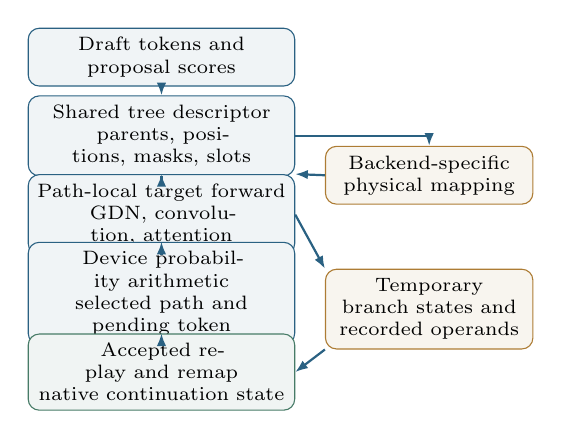
\begin{tikzpicture}[font=\scriptsize,
 box/.style={draw=inkblue,fill=inkblue!7,rounded corners,align=center,text width=3.15cm,minimum height=0.62cm},
 side/.style={box,text width=2.4cm,draw=mutedamber,fill=mutedamber!8},
 arr/.style={-{Latex[length=1.6mm]},thick,draw=inkblue}]
\node[box] (draft) at (0,0) {Draft tokens and proposal scores};
\node[box] (desc) at (0,-1.0) {Shared tree descriptor\\parents, positions, masks, slots};
\node[box] (verify) at (0,-2.0) {Path-local target forward\\GDN, convolution, attention};
\node[box] (select) at (0,-3.0) {Device probability arithmetic\\selected path and pending token};
\node[box,draw=mutedgreen,fill=mutedgreen!8] (commit) at (0,-4.0) {Accepted replay and remap\\native continuation state};
\foreach \a/\b in {draft/desc,desc/verify,verify/select,select/commit} \draw[arr] (\a)--(\b);
\node[side] (layout) at (3.4,-1.5) {Backend-specific physical mapping};
\node[side] (scratch) at (3.4,-3.2) {Temporary branch states and recorded operands};
\draw[arr] (desc.east) -| (layout.north);
\draw[arr] (layout.west) -- (verify.north east);
\draw[arr] (verify.east) -- (scratch.north west);
\draw[arr] (scratch.south west) -- (commit.east);
\end{tikzpicture}

\caption{The tree verifier as a serving pipeline. A shared descriptor connects candidate generation, ancestry-aware target computation, device probability arithmetic, and accepted-path publication. The attention backend determines the physical mapping; all state surfaces must describe the same selected prefix.}
\label{fig:pipeline}
\end{figure}

The paper develops three implementation contributions. \textit{First}, it presents the integrated verifier architecture and its continuation interface: candidates follow their ancestors during verification, and the selected materialized path becomes the next native state. \textit{Second}, it explains the GPU scan/replay design, including its shared update, branch-state workspace, accepted-path publication, and memory--recomputation tradeoff. \textit{Third}, it organizes the implemented optimizations around the work they remove and the numerical and backend constraints they must preserve: draft-logit reuse, device probability arithmetic, vectorized convolution, packed operands, attention layout/grouping, and scan/acceptance batching. We distinguish implemented candidates from the components active in the fresh measured route and from independently measured optimization gains.

The evaluation supports this design account with fresh same-input arithmetic comparisons, bounded continuation checks, eighteen configuration-comparison boots, and six additional boots for a qualified draft-logit-reuse ablation. Local triangular-solve and finite-Neumann realizations probe alternatives to sequential scan/replay; neither passes all frozen promotion criteria. The measured tree configuration exceeds the longer native chain but trails the depth-comparable native chain, with output divergence and an engine-seed difference disclosed. The separate reuse ablation measures the effect of avoiding a redundant vocabulary projection within the tree route; it does not replace the native/tree comparison. These results characterize the implemented configurations rather than establishing a general acceleration or quality-preservation claim.

Tree verification and compact accepted-state reconstruction have direct prior art. Section~\ref{sec:related} positions our implementation against those mechanisms; we do not claim the first hybrid-tree system or a new GDN recurrence. The architecture and kernel design are developed in Sections~\ref{sec:contract}--\ref{sec:kernel}, and Section~\ref{sec:optimization} separates optimization mechanisms from their measured scope. Measurement provenance is documented in Appendix~\ref{app:audit}; historical quantitative results are excluded throughout.

\section{Background and Related Work}
\label{sec:related}
\subsection{Drafting, verification, and serving}
Speculative sampling constructs an exact target sample from proposal and residual distributions, conditional on the probabilities actually supplied~\cite{leviathan2023fast,chen2023sampling}. SpecInfer supplies the tree-verification framing; Sequoia, EAGLE-2, and OPT-Tree investigate tree construction and its performance consequences~\cite{miao2023specinfer,chen2024sequoia,li2024eagle,wang2024opt}. Our study keeps these algorithmic questions separate from whether a deployed kernel and cache return the intended probabilities.

PagedAttention and SGLang address the scheduling, memory, and execution substrate~\cite{kwon2023efficient,zheng2024sglang}. Hybrid serving additionally manages recurrent-state pools alongside KV storage, as documented by SGLang's hybrid-model integration~\cite{pytorch2025sglang,sglang2026qwen}. Thus neither a fast isolated recurrent kernel nor low transient state memory alone determines user-visible latency. The measured native baseline uses FlashAttention while tree verification uses stock \texttt{TREE\_ATTN}; backend-specific work partitioning remains part of the execution boundary~\cite{dao2023flashattention,lumo2026archive}.

\subsection{Recurrent and hybrid speculation}
Gated DeltaNet augments a decayed recurrent state with a data-dependent delta update~\cite{yang2024gated}. Parallel delta-rule formulations provide relevant algebraic background~\cite{yang2024delta}. Stateful speculation is established territory: STree studies speculative trees for hybrid state-space models, SpecMamba targets an FPGA implementation, and component-aware self-speculation studies how hybrid components affect the design~\cite{wu2025stree,zhong2025specmamba,borobia2026component}. These works motivate an explicit state lineage; they do not justify treating every recurrent update or numerical implementation as interchangeable.

\subsection{Direct GDN comparisons}
\textbf{Bole} derives a tree-structured closed form and evaluates it with a value-tiled finite-polynomial solver. It stores compact update factors and reconstructs the accepted state. Its SGLang integration combines batch-wide verification budgeting with captured GPU execution. Evaluation includes unquantized Qwen3.5-27B on GB10 and online replay of agent sessions~\cite{wang2026bole}. Its state and serving mechanisms directly overlap the problem studied here. The cost of our replay implementation is not a lower bound on alternatives.

Concretely, Bole's correction system is $(I+G)U=R$, where $G$ contains strict-ancestor interactions and $R$ is the source correction. Tree depth $d$ gives $G^{d+1}=0$, so $U=\sum_{m=0}^{d}(-G)^mR$. This finite identity changes the arithmetic schedule from sequential updates to matrix propagation~\cite{wang2026bole}. Our path preserves sequential updates and replays accepted operands; Section~\ref{sec:reconstruction-numerics} explains why the numerical comparison remains an empirical question.

\textbf{TreeWY} expresses GDN tree verification as a triangular system and reconstructs the accepted state from pseudo-values. Its vLLM evaluation uses Qwen3.5-35B and 397B on B200, greedy verification, and disabled prefix caching. It explicitly permits finite-precision disagreement with the baseline and reports that wider trees improve acceptance without yet winning throughput~\cite{ghantasala2026treewy}. Consequently, our local numerical comparisons neither establish that TreeWY is incorrect nor replace its serving comparison.

\textbf{ReplaySSM} caches recurrent inputs and changes when state is materialized; its implementation RFC includes GDN and Mamba2~\cite{replayssm2026}. Reconstruction and replay are not claimed as new concepts here. Table~\ref{tab:related} states the comparison boundary. Published speed ratios from different checkpoints, precision formats, workloads, and software builds are not combined into a performance ranking.

\begin{table}[t]
\caption{Direct comparison scope. External methods were read, not executed in this revision.}
\label{tab:related}
\centering\footnotesize
\begin{tabularx}{\columnwidth}{@{}>{\raggedright\arraybackslash}p{0.22\columnwidth}YY@{}}
\toprule
Method & Overlapping mechanism & Boundary for this study \\
\midrule
Bole~\cite{wang2026bole} & Parallel verifier; factorized commit & Different stack and precision; no matched run \\
TreeWY~\cite{ghantasala2026treewy} & Tree solve; accepted-state reconstruction & Different models and operating regime; no matched run \\
ReplaySSM~\cite{replayssm2026} & Input caching; deferred state work & Alternative state policy; no matched run \\
\sys{} & Scan/replay; accepted-path remapping & Specific numerical and lifecycle witnesses; scoped cost evidence \\
\bottomrule
\end{tabularx}
\end{table}

\section{Tree-Verifier Architecture}
\label{sec:contract}
\subsection{State and the execution boundary}
Let $m$ be a materialized token prefix: the tokens already consumed by the target's forward computation. Write its persistent state as
\begin{equation}
\mathcal{S}(m)=\bigl(R(m),C(m),K(m)\bigr),
\end{equation}
where $R$ collects recurrent matrices, $C$ collects convolution histories, and $K$ collects attention KV entries. The logical emitted prefix can also include a newly sampled token $b$ that has not yet been consumed. The continuation boundary is then $(\mathcal{S}(m),b)$, not a claim that $\mathcal{S}(mb)$ has already been computed. This distinction is essential when counting the correction or bonus token while checking cache state.

A tree descriptor contains candidate token IDs, parent indices, depth/position information, attention visibility, and maps between logical nodes and physical slots. For a candidate node $i$, each target layer must consume the state obtained from the candidate's root-to-parent path. At publication, the selected materialized path, pending-token convention, and next-drafter input row must agree. Figure~\ref{fig:contract} illustrates the three state surfaces documented by the implementation audit~\cite{lumo2026stateless,lumo2026archive}.

\subsection{The recurrence and path locality}
For one GDN head, let $R\in\mathbb{R}^{d_v\times d_k}$. Queries and keys are in $\mathbb{R}^{d_k}$ and values in $\mathbb{R}^{d_v}$. With decay $\alpha_i$ and write strength $\beta_i$, a node applies the standard update~\cite{yang2024gated}
\begin{align}
R'_i &= \alpha_i R_{\pi(i)}, &
\delta_i &= \beta_i\bigl(v_i-R'_i k_i\bigr),\\
R_i &= R'_i+\delta_i k_i^\top, &
o_i &= R_iq_i,
\end{align}
where $\pi(i)$ is its parent. A previous node in the packed buffer need not be $\pi(i)$. The causal convolution likewise requires path predecessors rather than adjacent packed rows. The attention visibility relation must select the same logical prefix and ancestry. These requirements follow from the model's computation; a correct attention mask cannot repair a wrong recurrent parent.

The implementation verifies nodes with branch-local scratch and makes the selected continuation durable through replay and remapping. This is an implementation route, not the only way to satisfy the contract~\cite{lumo2026archive,lumo2026stateless}. In particular, rejecting a branch requires that its contents cannot influence future computation; it does not require zeroing every scratch byte if future reads are correctly restricted.

\subsection{A descriptor shared by verification and commitment}
Figure~\ref{fig:pipeline} shows the served path. Native multi-token prediction (MTP) supplies the principal draft chain; selected variants add runner-up candidates. The descriptor maps each candidate through the attention mask, recurrent scan, sampler, and selected-path publication. The evaluated Cat10 descriptor contains the root and nine MTP draft nodes, with a maximum draft-path depth of five~\cite{lumo2026archive}.

\begin{figure}[t]
\centering
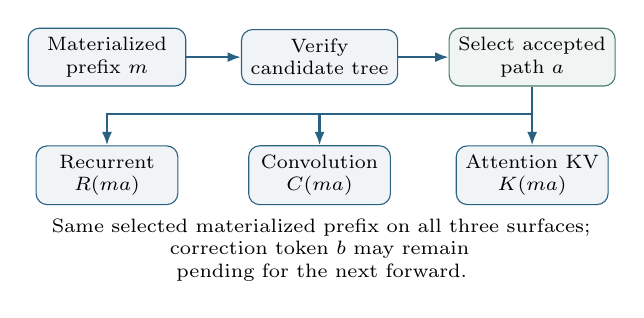
\begin{tikzpicture}[font=\scriptsize,
 box/.style={draw=inkblue,fill=inkblue!7,rounded corners,align=center,minimum height=0.7cm},
 arr/.style={-{Latex[length=1.7mm]},thick,draw=inkblue}]
\node[box,minimum width=2.0cm] (prefix) at (0,0) {Materialized\\prefix $m$};
\node[box,minimum width=1.8cm] (tree) at (2.7,0) {Verify\\candidate tree};
\node[box,draw=mutedgreen,fill=mutedgreen!8,minimum width=2.0cm] (path) at (5.4,0) {Select accepted\\path $a$};
\draw[arr] (prefix)--(tree);\draw[arr] (tree)--(path);
\node[box,minimum width=1.8cm] (r) at (0,-1.5) {Recurrent\\$R(ma)$};
\node[box,minimum width=1.8cm] (c) at (2.7,-1.5) {Convolution\\$C(ma)$};
\node[box,minimum width=1.8cm] (k) at (5.4,-1.5) {Attention KV\\$K(ma)$};
\draw[arr] (path.south) -- ++(0,-0.35) -| (r.north);
\draw[arr] (path.south) -- ++(0,-0.35) -| (c.north);
\draw[arr] (path.south)--(k.north);
\node[align=center,text width=7cm] at (2.7,-2.45) {Same selected materialized prefix on all three surfaces;\\correction token $b$ may remain pending for the next forward.};
\end{tikzpicture}

\caption{The accepted-prefix interface. Recurrent, convolution, and attention-KV state must all describe the same materialized prefix. A newly sampled correction or bonus token can remain pending until the next forward.}
\label{fig:contract}
\end{figure}

The evaluated stock \texttt{TREE\_ATTN} route uses flat candidate slots and the descriptor's ancestry mask. Its cache-write addresses, attention-read addresses, and accepted-path remapping share that flat node convention. Recurrent nodes obtain their parent state from the pre-tree state or node-local scratch. After device selection, accepted-path replay and remapping establish the continuation state~\cite{lumo2026archive}. Cache checkpoints and restored rows must obey the same contract; a correct cold first request does not establish correctness after a checkpoint hit or page reuse~\cite{lumo2026stateless}.

\begin{algorithm}[t]
\caption{Logical verifier and continuation boundary}
\label{alg:verify}
\begin{algorithmic}[1]
\REQUIRE Reference-aligned state boundary, candidate descriptor $T$
\STATE Map logical candidates to physical slots and positions.
\STATE Verify using path-local convolution, GDN, and attention.
\STATE Apply the configured sampler to matching target/proposal rows.
\STATE Obtain the accepted path and any pending correction token.
\STATE Publish recurrent and convolution state for the materialized path.
\STATE Map its attention KV entries to the native continuation layout.
\STATE Map the selected hidden-state row to the next drafter input.
\STATE Preserve the native pending-token and position convention.
\RETURN Continuation boundary and emitted-token accounting
\end{algorithmic}
\end{algorithm}

\section{GPU Scan and Accepted-Path Replay}
\label{sec:kernel}
\subsection{Verification workspace and native state lifetime}
The branch-local scan evaluates nodes in a topological order. A root candidate starts from the pre-tree state; another node starts from its parent's post-state. Packed adjacency alone supplies neither relationship. The cached implementation keeps node post-states in a tile-local table while writing the candidate outputs used by later layers. A separate activation ring records the operands needed to replay the chosen path after acceptance~\cite{lumo2026archive}.

This workspace is speculative. The stateless serving route initializes it from request-owned native running rows and publishes the accepted state back to those rows. Recurrent and convolution publication must agree, since a later continuation or native cache operation can read both surfaces. Speculative scratch is retired by the selected lifecycle; no persistent leaf selector is needed to locate the next request state~\cite{lumo2026stateless}. This is a state-management design, not a claim that speculative workspace consumes no memory. Fresh validation covers the selected eager route with prefix caching disabled, not every restore/eviction path.

\begin{algorithm}[t]
\caption{Logical scan and selected-path publication; compiled loops may include masked padding.}
\label{alg:scan-replay}
\begin{algorithmic}[1]
\REQUIRE Pre-tree state $R_0$, descriptor $T$, rounded node operands $x_i$
\FOR{node $i$ in topological order}
\STATE $R_p\gets R_0$ if $i$ has no candidate parent; otherwise $R_p\gets H[\pi(i)]$
\STATE $(H[i],o_i)\gets\operatorname{NodeStep}(R_p,x_i)$
\ENDFOR
\STATE Finish target forward and select accepted materialized path $A$
\STATE $R\gets R_0$
\FOR{node $i$ in $A$, in path order}
\STATE $(R,\_)\gets\operatorname{NodeStep}(R,x_i)$
\ENDFOR
\STATE Publish $R$ and matching convolution history to native running rows
\STATE Remap accepted KV entries and retire speculative scratch
\RETURN Matching continuation state and any pending token
\end{algorithmic}
\end{algorithm}

\subsection{A shared update with explicit rounding boundaries}
Scan and replay call the same node-update body. Replay consumes the accepted path's recorded operands in order, so it does not reconstruct the final state from an unrelated rounded output representation. The source exposes choices for raw-gate evaluation, query/key normalization, beta rounding, output storage, and carried-state precision. These choices must be pinned to a particular reference: the native speculative-update kernel and repeated one-token decode are distinct numerical references~\cite{lumo2026archive}.

Sharing source makes the intended arithmetic common; it does not by itself guarantee identical compiled instructions. Operand shapes, launch geometry, unrolling, and compiler scheduling can change reduction or contraction order. We therefore separate the real-arithmetic recurrence from comparisons of compiled outputs and committed states. Section~\ref{sec:e7a-pilot} evaluates these quantities independently on the same fresh operands, and Section~\ref{sec:selected-route} checks whether the next invocation consumes the state actually published.

\subsection{Caching, replay, and recomputation}
Let $N_p$ be the padded node span, $B_v$ the value-tile width, and $d_k$ the key dimension. A cached scan's fp32 node-state table has logical footprint
\begin{equation}
 M_H = 4N_pB_vd_k\ \text{bytes per program}.
\end{equation}
For $W$ warps, $N_pB_vd_k/(32W)$ is a useful estimate of cached fp32 values per lane, before live operands and compiler allocation. This is a resource model, not a measurement of allocated registers or spills. Padding can increase workspace even when the additional rows do not represent useful candidates. Narrower tiles reduce the state table but create more programs and can alter the numerical execution layout.

Accepted-path replay instead carries one state tile and traverses a loop bounded by the configured path capacity, masking unused positions. Its selected-path semantics do not imply that arithmetic or latency scales only with the number of accepted nodes. Its carried-state footprint is $O(B_vd_k)$ in tree size, although recorded operands and the broader serving scratch still scale with candidates. Verification variants can similarly recompute a node's ancestry or divide the tree into paths rather than retaining every node post-state. This exchanges stored state for repeated recurrence work; the useful choice depends on topology and GPU resource pressure~\cite{lumo2026archive}. None of these analytic footprints is a reported historical performance result.

\begin{figure}[t]
\centering
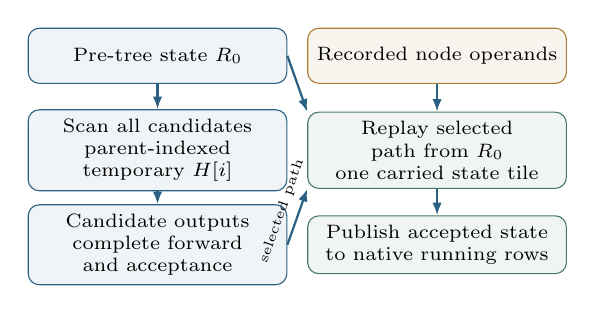
\begin{tikzpicture}[font=\scriptsize,
 box/.style={draw=inkblue,fill=inkblue!7,rounded corners,align=center,text width=3.05cm,minimum height=0.7cm},
 arr/.style={-{Latex[length=1.6mm]},thick,draw=inkblue}]
\node[box] (prior) at (0,0) {Pre-tree state $R_0$};
\node[box] (scan) at (0,-1.2) {Scan all candidates\\parent-indexed temporary $H[i]$};
\node[box] (out) at (0,-2.4) {Candidate outputs\\complete forward and acceptance};
\node[box,draw=mutedamber,fill=mutedamber!8] (ring) at (3.55,0) {Recorded node operands};
\node[box,draw=mutedgreen,fill=mutedgreen!8] (replay) at (3.55,-1.2) {Replay selected path from $R_0$\\one carried state tile};
\node[box,draw=mutedgreen,fill=mutedgreen!8] (publish) at (3.55,-2.4) {Publish accepted state\\to native running rows};
\draw[arr] (prior)--(scan);
\draw[arr] (scan)--(out);
\draw[arr] (ring)--(replay);
\draw[arr] (prior.east)--(replay.north west);
\draw[arr] (out.east)--node[above,sloped,font=\tiny]{selected path}(replay.south west);
\draw[arr] (replay)--(publish);
\end{tikzpicture}

\caption{Different state lifetimes within one verification step. The cached scan uses parent-indexed temporary states to produce candidate outputs. Accepted-path replay starts again from the pre-tree state and publishes only the chosen continuation. Compact reconstruction is a separately evaluated alternative.}
\label{fig:scan-replay}
\end{figure}

Compact triangular-solve and finite-Neumann methods choose another point in this design space: they form correction factors and reconstruct the accepted state without replaying every accepted rank-one update. Our local comparison evaluates their verifier arithmetic and state reconstruction separately. Lower state-storage requirements or less replay work alone do not establish lower complete-step latency, and numerical agreement must be assessed at the actual output and state-storage boundaries~\cite{ghantasala2026treewy,wang2026bole}.

\section{Optimization Mechanisms and Backend Constraints}
\label{sec:optimization}
\subsection{Reuse draft logits and keep probability arithmetic on device}
The native-MTP drafter supplies both a principal spine token and runner-up candidates from the same logits tensor. The single-logits path selects the spine token from that existing tensor, avoiding a second vocabulary projection inside the native greedy-sampling helper. Both the reuse path and its counterfactual OFF control obtain runner-up candidates from the first logits; the redundant work is the second projection for spine selection. Runner-up leaves use these scores without advancing an independent drafter state for each leaf. The descriptor keeps this proposal policy separate from target verification, allowing a different drafter to supply the same interface~\cite{lumo2026archive}. Reusing scores does not establish that a wider tree yields a net serving gain: its additional target rows still cost work.

The device multidraft committer keeps target/proposal probability arithmetic and residual selection on GPU tensors, avoiding a full-vocabulary probability transfer to the host. The active fresh route still has Python request/node control loops and scalar readbacks; device-resident arithmetic is not a fully device-resident acceptance walk. The selected node sequence drives recurrent replay, convolution publication, KV remapping, and the next drafter's hidden-row selection~\cite{lumo2026archive}. Greedy longest-prefix selection is not a substitute for a stochastic residual rule. The fresh campaign's temperature-zero path checks establish only their stated greedy and continuation scope.

\subsection{Prepare convolution rows and replay operands together}
Tree convolution must gather a different causal window for each candidate path. The vectorized implementation builds static source indices over the prior history, current node inputs, and a zero row, then gathers the needed windows and state rows. Its tap computation uses explicit ordered additions and matching cast boundaries instead of replacing the original order with an unconstrained reduction. Preparing accepted-path row indices once per state group also avoids rebuilding the same mapping independently in each layer~\cite{lumo2026archive}.

This vectorized convolution route and the eager packed-buffer preparation are active in the fresh implementation. The latter organizes recorded operands across layers and prepares shared metadata. Buffer packing and replay launch batching remain different mechanisms: the fresh greedy route follows canonical multidraft acceptance, whose unarmed replay branch still iterates over layers. The existence of stacked buffers therefore does not establish that all-layer replay was executed or that all replay launches were removed. Table~\ref{tab:optimization-map} records this distinction; no isolated timing gain is assigned to either component.

\subsection{Launch organization and independent acceptance work}
The repository also implements candidates that fold independent GDN work into fewer launches and batch tree-acceptance work across requests. These attack launch overhead and underfilled device work, respectively. They retain per-request ancestry and output identities; a batching change must also preserve the intended normalization and cumulative-sum behavior. Attention grouping/padding candidates target reuse and execution geometry in the FA2 route. These are source-level optimization mechanisms, not automatically components of every tree configuration~\cite{lumo2026archive}.

Table~\ref{tab:optimization-map} separates this design inventory from the fresh evidence. In particular, the fixed-shape scan and acceptance candidates cannot be treated as simple enabled optimizations of the fresh caterpillar route without checking their shape, backend, and launcher guards. The present fresh whole-configuration timing does not measure their individual or composed gains.

\begin{table*}[t]
\caption{Optimization-to-evidence map. ``Implemented'' describes source availability; it does not assert a fresh isolated speedup or activation in every serving route.}
\label{tab:optimization-map}
\centering\footnotesize
\begin{tabularx}{\textwidth}{@{}p{0.20\textwidth}p{0.28\textwidth}YY@{}}
\toprule
Mechanism & Work or dependency addressed & Implementation boundary & Fresh evidence / missing ablation \\
\midrule
Draft-logit reuse & Share one vocabulary projection for spine selection and runner-up candidates & Active in E1; source-controlled ON/OFF variants in E8 & Qualified same-input checks and six B1 timing boots (Section~\ref{sec:e8-timing}) \\
Device probability arithmetic & Avoid full-vocabulary host transfer & Active; Python control and scalar readbacks remain & Bounded selected-path checks; no device/host latency ablation \\
Vectorized tree convolution & Reuse static path-window indices and ordered tap operations & Active tree-only helper path & No fresh fused/legacy latency ablation \\
Packed eager buffers & Share operand storage and metadata preparation & Active; canonical replay still loops over layers & All-layer replay must not be inferred from buffer engagement \\
Scan/replay state policy & Temporary branch states; publish only accepted native state & Shared node update, activation ring, running-row lifecycle & Fresh arithmetic and continuation checks; state-policy performance ablation absent \\
Accepted-path KV remap & Publish selected continuation addresses & Active with flat slots and sync-free remap; slot reordering disabled & Fresh incompatible-policy control and selected-route checks \\
Attention grouping/padding & Change work grouping and reuse & Forked-FA2 configuration, not fresh stock \texttt{TREE\_ATTN} & No fresh isolated or composed timing \\
Single-launch scan / batched acceptance & Reduce launch overhead / combine independent request work & Fixed-shape candidate routes; compatibility gate required & No fresh composed optimization result \\
\bottomrule
\end{tabularx}
\end{table*}

\subsection{Publish the selected path in the backend's address space}
The current continuation path copies accepted attention KV entries from their verification slots into linear continuation slots. If accepted logical node $a_j$ becomes continuation position $j$, the remapper moves its KV entry from the descriptor's source slot for $a_j$ to the request's native destination slot for $j$. Recurrent replay, convolution publication, and the next drafter row use the same selected path. KV publication is state movement; it does not change the attention equation~\cite{lumo2026archive}.

For the measured stock \texttt{TREE\_ATTN} backend, verification writes and attention reads retain flat candidate positions. The selected route enables accepted-path KV remapping and its sync-free helper, leaves slot reordering disabled, and uses synchronous scheduling. A layout permutation is valid only when both read and write mappings, ancestry visibility, and continuation publication use the same convention. Section~\ref{sec:selected-route} reports the fresh incompatible-policy control and the checks of this selected flat-map implementation. The artifact binds effective post-boot settings to loaded source, so source availability alone is not treated as engagement.

\subsection{Reconstruction, rounding, and accumulated disagreement}
\label{sec:reconstruction-numerics}
Verification outputs, committed state, and later model outputs are separate numerical boundaries. A first-order explanatory model is $e_{\ell+1}\approx J_\ell e_\ell+\delta_\ell$: later layers can amplify an existing residual while introducing additional error. This expression is not a fitted error bound. Small local errors, or matching current outputs, do not establish matching future logits. The fresh same-input and continuation studies below therefore evaluate verification arithmetic and state publication separately.

The numerical reference must also be named. The pinned native speculative-update and one-token decode paths differ in gate rounding and state-storage boundaries. Our scan and replay share a sequential update body, but their compiled agreement still requires GPU checks~\cite{lumo2026archive}. Thus a real-arithmetic reconstruction identity does not by itself establish deployment agreement; conversely, disagreement with our selected reference does not establish an algebraic defect. E7a and E7b isolate verification arithmetic, state commitment, and subsequent continuation before measuring any deployment benefit. E7a explicitly tests the native paths' rounding conventions on fresh captured operands (Section~\ref{sec:e7a-pilot}); their different state-storage rules remain distinct reference contracts.

\section{Evaluation Setup}
\label{sec:protocol}
The evaluation asks how the sequential implementation compares with compact arithmetic on identical operands, whether selected continuation state is consumed correctly, and how the measured serving configurations perform. The main stack is Qwen3.6-27B-FP8 on GB10/DGX Spark~\cite{qwen2026qwen36fp8,lumo2026archive}. Table~\ref{tab:evidence} separates kernel measurements, stage substitutions, route qualification, and timing; their instrumentation differs and they are not interchangeable replicates.

The selected fresh tree configuration uses stock \texttt{TREE\_ATTN}, flat candidate slots, accepted-path attention-KV remapping, eager execution, synchronous scheduling, and disabled prefix caching. This defines the measured implementation, not the whole optimization inventory in Table~\ref{tab:optimization-map}. The timing study evaluates fixed qualified configurations; it does not search for the fastest deployment of either native MTP or the tree verifier. Numerical results use fresh captures or explicitly labeled fresh synthetic controls. Historical results and remeasurements on archived operands are excluded. The artifact retains exact source identities, original failures, and immutable campaign records; Appendix~\ref{app:audit} explains the measurement reconciliation.

\begin{table*}[t]
\caption{Evidence from the current revision. P0, E7a, bounded E7b diagnostics, selected-route E2 checks, eighteen E1 timing cells, and six E8 component-ablation cells are executed. Historical findings appear only as qualitative background; E3 remains conditional and E7c deferred.}
\label{tab:evidence}
\centering\footnotesize
\begin{tabularx}{\textwidth}{@{}p{0.05\textwidth}p{0.17\textwidth}Yp{0.25\textwidth}@{}}
\toprule
ID & Evidence & Supported statement & Important boundary \\
\midrule
P0 & Configuration audit (Appendix~\ref{app:audit}) & Sampling reconstruction; no new model measurements & Historical binary gaps retained \\
E7a & Same-input kernel study (Section~\ref{sec:e7a-pilot}) & Fresh synthetic controls, eight fresh pilot prefixes, and 31 of 32 confirmation prefixes passing the frozen provenance checks & Local realizations, not the authors' systems; frozen numerical/control criteria missed; no model-level qualification \\
E2/E7b & Stage-isolated and selected-route checks (Sections~\ref{sec:e7b-diagnostic}--\ref{sec:selected-route}) & One-prefix propagation diagnostics and bounded B1/B4 serving-contract evidence & No live conv/KV byte snapshots, full-model sequential-equivalence or general sampler-law proof \\
E1 & Eighteen fresh timing boots (Section~\ref{sec:e1-timing}) & Three configurations, B1/B4, three paired blocks; exact token/wall support & Different continuations and engine seeds; coarse uncertainty; as-executed comparison \\
E8 & Six fresh single-logits ON/OFF boots (Section~\ref{sec:e8-timing}) & Common engine/API seed, same-input head qualification, and measured B1 component contrast & Three paired blocks; different continuations in the final ON boot; no B4 or composed gain \\
E3 & Conditional; not promoted & --- & No composed optimization result \\
\bottomrule
\end{tabularx}
\end{table*}

\section{Results}
\label{sec:results}
\subsection{E7a: arithmetic on fresh operands and synthetic controls}
\label{sec:e7a-pilot}
The final confirmation study retains 31 provenance-passing inputs from 32 frozen prefixes and does not satisfy all original promotion criteria. Neither compact candidate is promoted. The pilot observations below explain the frozen choices; the subsequent confirmation and completed audit determine this final verdict.

E7a uses the rounded operands of one GDN layer step: bfloat16 $q,k,v$, bfloat16 raw gates, fp32 $A_{\log}$, bfloat16 gate bias, the fp32 pre-tree state, and the tree descriptor. Three references remain distinct: a float64 serial recurrence on the same rounded operands, the pinned native speculative-update kernel run per root-to-node chain, and the pinned one-token decode kernel run token by token. We report the revision's fresh pilot and confirmation captures below, with a separately labeled fresh synthetic stress test. Preliminary remeasurements on archived captures and legacy kernels remain outside the manuscript's quantitative results.

A fresh eight-prefix pilot ran on 22 September 2026 on the intended configuration: the audited Qwen3.6-27B FP8 checkpoint (read-only), the pinned vLLM image, B1 eager execution with stock \texttt{TREE\_ATTN}, and the served ten-node caterpillar on the stateless production tree route (distinct from the archived forked FlashAttention-2 route), and a documented one-hunk repair of the source patcher that made that route runnable at HEAD (a drafter constant emitted only under a fixed-tree mode; recorded with original and repaired hashes). Ninety-six candidate prefixes were cut from local repositories in three context strata and scored once by a native MTP reference server; eight pilot and 32 disjoint confirmation prefixes were frozen from native-reference behavior alone (top-1/top-2 margin and context strata) before any tree output was read. Each pilot prefix received one boot and one greedy request, and one one-shot capture of layer 62's first tree step after the full prefill (two prefill forwards for the 4096-token prompts under the server's logged 2048-token budget). A fail-closed provenance inspector (51 checks per capture: hashed prefix and prompt-token binding, payload written inside the first tree step, the per-request scheduler trace carrying the response identifier, per-step alignment of the accepted draft paths with the API-returned token identifiers, exact decoding of those identifiers to the response text, exact geometry and dtypes, non-trivial pre-state) passed on all eight (four prompts of 256 tokens, four of 4096), with three earlier boots retained as failed captures. The eight sets are independent frozen prefixes; the harness run of record is \path{experiments/out-20260922T013313Z-e7a-fresh-pilot-v2/}.

Mechanism A is this worktree's production scan and accepted-path replay. Mechanisms B and C are our Triton reimplementations of the two published families on the same masked system $(I+G)U=R$: forward substitution (the WY/TreeWY family) and the finite Neumann series $\sum_{m=0}^{d}(-G)^mR$ ($d$ correction powers plus the identity, hence $d+1$ terms; the Bole family), each followed by the compact reconstruction $S_a=P_aS_0+\sum_{j\preceq a}(P_a/P_j)\,u_jk_j^\top$. Dense products run either in fp32 or in tf32 tensor-core precision. Every accepted prefix, including zero acceptance, is committed, first from each method's own factors and then from identical oracle factors.

A fresh synthetic tiny-gate pass (\path{out-20260921T231030Z-e7a-tinygates-v3/}; chains of depth 11 and 5 and the caterpillar with cumulative log-decay down to $-912$, so that the path decay $P_i$ underflows to exactly zero in fp32) produced no non-finite value in any realization. With fp32 dense products, the diagnostic fp32-output-store outputs and committed fp32 states stayed within $0.9$--$5.8\times10^{-7}$ relative to the corresponding oracle maximum. Every implementation evaluates path-decay ratios as $\exp(\log P_i-\log P_j)$ with the exponent masked before exponentiation, never as a literal quotient of underflowed products. The same run shows that with vanishing gates the strict-ancestor coupling vanishes too, so even the truncated Neumann series is accurate there; the truncation control fails only when coupling is present.

The eight-prefix pilot determined the candidate precision modes and frozen comparison rules. Before reading confirmation outputs, we selected A, B, and C with fp32 dense products; fixed each numerical tolerance from the corresponding pilot maximum and a declared margin; specified zero units in the last place for bitwise classes; and fixed the decision changes that would alter the claims. The verify-kernel timing rule required a relative half-width of at most 5\%; sub-20-microsecond commit kernels were reported without that gate. The resampling unit was the frozen prefix. Pilot-only passing observations and kernel timings are retained in the artifact as developmental evidence; the confirmation results and completed audit below govern the reported numerical verdict.

The confirmation set (artifacts of record \path{experiments/out-20260922T051611Z-e7a-fresh-confirmation/}) contains 32 disjoint frozen prefixes, sixteen each with 256 and 4096 prompt tokens. One boot hung after autotuning and was retried after the driver's timeout. One captured prefix, p087, failed the frozen provenance inspector: duplicate-token siblings made its path walk choose a different node from the served committer. That failure remains in the 32-prefix denominator. A revised path-consistency inspector passes the capture retrospectively; it does not replace the original verdict or add p087 to the 31-set primary comparison.

On the 31 provenance-passing sets, the production scan's fp32-store output is bit-identical to the native speculative-update kernel's, and the served bfloat16 output is byte-identical to the production scan's. The maximum absolute compact-commit state errors are approximately $7.81\times10^{-7}$ against the oracle and $1.91\times10^{-6}$ against native; replay maxima are $1.34\times10^{-6}$ and $2.38\times10^{-7}$, respectively (rounded). B and C's bfloat16 outputs agree with native on at least 99.9772\% of elements (the minimum is C on p005, with 14 of 61,440 elements differing). The served output is within $4.9\times10^{-4}$ of the oracle and within one bfloat16 unit in the last place on significant elements. Sibling reordering and repeat replay remain bitwise invariant in their tested controls.

The frozen criteria are not satisfied. Native and production bfloat16 stores differ in one element on each of two sets, despite identical fp32 stores. One set exceeds the frozen absolute output tolerance by 3\% ($9.2\times10^{-8}$ versus $8.9\times10^{-8}$). The frozen ordering $A\le B=C$ for output error fails on three sets, and B/C compact-state error equality fails on p031 by $6.9\times10^{-8}$. Padding from 16 to 32 nodes changes output and correction-factor bits for B and C on all 31 sets. Timing also misses both declared checks: three blocks exceed 5\% probe drift, and 14 verify-kernel timing cells across 12 prefixes exceed the 5\% relative half-width limit, reaching 32.09\%. Here ``relative half-width'' means $(p_{90}-p_{10})/(2\,\mathrm{median})$ across repeated kernel timings, a dispersion measure rather than a confidence interval.

A retrospective completeness audit found that the first checker omitted padding, compact-state ordering, and timing half-width checks. The immutable freeze also incorrectly described the pilot as padding invariant and timing compliant: the referenced fresh-pilot-v2 data already fail padding on all eight prefixes and the half-width limit in seven timing cells across six prefixes (maximum 20.23\%). We retain the original freeze and reports and record the corrections separately in \path{p0/monitor/2026-09-22-review-14-frozen-audit.json}. This is an audit of a flawed frozen analysis, not a corrected preregistration. These observations characterize the captured arithmetic; they do not qualify deployment, establish model-level harmlessness, or promote either compact route.

\subsection{Stage-isolated model diagnostics}
\label{sec:e7b-diagnostic}
We next isolated verifier substitution on one frozen pilot prefix, p072, at B1 with eager execution and the same pinned FP8 stack. Three separate boots ran the instrumented production route, a matched sham that computed B's fp32 forward-substitution result without publishing it, and a verifier-only arm that published that result at layer 62. All three passed provenance checks. Across twelve contiguous, input-aligned steps with ten candidate rows each, the production and sham captures had identical logits, hidden states, residuals, and emitted token sequences. The thirteenth capture was partial at the response boundary and was excluded from the aligned comparison. This pair's agreement is a control observation, not a universal cross-boot noise floor.

Against that sham, substitution first changed layer 62 and then layer 63; layers 0--61 remained identical. The largest absolute final-logit differences were 0.15625 at step 3 and 0.125 at step 7. No argmax changed among the 120 matched candidate rows, and all 32 emitted tokens were unchanged. Across thirteen verifier invocations, the minimum local bfloat16-output equality fraction was 99.9788\%, with a maximum absolute difference of $6.10\times10^{-5}$. These observations demonstrate propagation in this implementation and prefix, without establishing model-level harmlessness or a defect inherent to either published mechanism. Raw captures and the independently checked reduction are retained under \path{experiments/out-20260922T063019Z-e7b-r13-p072-batch/}.

An independent review also found a publication defect in the diagnostic commit hook: on paths with more than one accepted draft, replacing only the accepted-column copy left the authoritative running state unchanged when the next forward read column zero. That defect concerns our substitution harness, not the compact algebra. After repair, three new boots ran production, a matched commit sham, and B's commit-only substitution on p072 (\path{experiments/out-20260922T071945Z-e7b-r16-p072-commit-batch/}). Production and sham captures were bit-identical, including their 32 emitted tokens. All thirteen compact publications changed the authoritative state; all twelve captured next-forward pre-states consumed the preceding published bytes exactly. Across twelve input-aligned verifier calls, the compact arm changed final logits in two calls (maximum absolute difference 0.15625), without changing an argmax or the emitted token sequence. Only eleven calls had complete post-commit boundaries within the API output; the terminal partial call and extra capture are not additional fully emitted continuation intervals.

For a separate fixed-input check, we injected the compact arm's first published layer-62 state into an offline float64 recurrence using the sham's subsequent recorded operands and accepted paths, with fp32 state storage between steps. The initial maximum state difference, $2.38\times10^{-7}$, remained at that value over ten fully API-bound continuation intervals; maximum output differences ranged from $1.79\times10^{-9}$ to $4.85\times10^{-9}$. The production-to-sham control stayed exactly zero. This once-injected, one-layer experiment differs from the live arm's repeated compact commits and does not exercise cross-layer feedback. No amplification was observed in its tested maximum-state-error measure and horizon. All thirteen captured steps of the production and compact boots also met the declared layer-level numerical fidelity checks, and all twelve pre-state links were bit-identical to the prior publication. None of these checks qualifies convolution history, attention KV, the sampler law, or the full serving route; those surfaces remain separate E2 requirements. The recorded environments for all six diagnostic boots omit the plain-route attention-KV remap flag, whose loaded source defaults to disabled. Their local arithmetic and matched-arm observations therefore do not establish correct branch-path attention continuation; the corrected serving route is qualified separately in Section~\ref{sec:selected-route}.

\subsection{Backend-specific continuation checks}
\label{sec:selected-route}
Repairing attention continuation required checking both sides of the loaded backend's address contract. A candidate policy enabled KV remapping, spine-first slot reordering, and the sync-free remap helper together. In the loaded \texttt{TREE\_ATTN} backend, however, cache writes followed the permuted slot mapping while unified-attention reads used flat block-table positions and the original node mask. A source-derived address fixture showed that query node 3 read current-tree nodes $[0,1,4]$ instead of $[0,1,3]$. On p072, the candidate policy and flat-map control had identical input hidden states and positions, but first differed at layer 3, the first full-attention layer. The final-logit maximum absolute difference was 6.125, with one changed argmax row. This is an incompatibility between these implementation settings, not a defect in the GDN recurrence or a published tree-verification method.

The selected policy keeps flat node slots, enables attention-KV remapping and its sync-free helper, and explicitly disables asynchronous scheduling. In a corrected B1 boot, the first forward matched the earlier diagnostic flat-map control from this revision across all 64 hidden-state/residual pairs and final logits. Later continuations differed after branch acceptance; that control had KV remapping disabled and is not a continuation oracle. Twelve captured layer-62 publications and eleven next-forward links verified that the authoritative state was read byte for byte. Actual draft tokens, parent topology, and full-vocabulary logits reconstructed all 31 post-prefill API tokens along their accepted-plus-bonus paths. The initial prefill token had API/ledger and returned-logprob evidence, but no captured full-vocabulary logits. The 32-token API response was the exact prefix of 34 structural outputs, with truncation only at its final boundary. A sealed event ledger independently reconciled these outputs and eleven complete physical-step intervals. This capture boot was not a warmed timing cell.

Helper tests separately checked active recurrent rows, convolution-history remainder protection, pending-token consumption, accepted-node KV copying, and four-request isolation, including multi-block KV layouts and corruption controls. Loaded-source guards and call order connect these helper contracts to the selected route; they do not substitute for live convolution/KV byte snapshots or a full-model sequential oracle.

An actual four-request pilot used two 256-token and two 4096-token prefixes. All 53 captured layer-62 computations met the declared numerical classes, and all 49 available publication-to-next-input links matched byte for byte, including request-row compaction as other requests finished. Eight complete B4 forwards supplied 32 request blocks with full-logit, candidate, position, and published-path evidence, covering 85 structural output tokens; 83 fell within the returned API responses. The complete ledger reconciled all four 32-token responses and seven complete B4-to-B4 intervals. The client had omitted direct token-ID reporting: independent exhaustive inversion of the exact pinned tokenizer and context-sensitive API formatter recovered all 128 IDs uniquely over the model's 248,320 output IDs, without consulting the ledger or draft IDs. Original strings and the derived-ID sidecar are retained, and subsequent clients request IDs directly. These finite checks qualify the selected eager, cache-off, temperature-zero route for the timing protocol; they do not establish full-model sequential equivalence.

That pilot also exposed a distinction between greedy token choice and tree-node choice. Two sibling nodes proposed token 561 with equal overlap weights; the loaded sampler randomly selected a source child even at temperature zero. The published path $[1,3]$ validly emitted tokens $[13,561,8057]$, whereas another legal sibling choice would continue along $[1,2,4]$. A gate requiring the first, last, or longest matching path would therefore reject a legal execution. The repaired check validates the actual published ancestry, each accepted token against its parent's target argmax, the terminal bonus, and the absence of nonterminal premature stopping at a node with a matching child; API-budget clipping is allowed only at that request's final output boundary. Original gate failures and their corrections are retained. This finite path check does not prove distribution preservation for stochastic sampling.

\subsection{Qualified eager-configuration timing}
\label{sec:e1-timing}
The timing experiment compares three instrumented configurations of the pinned Qwen3.6-27B-FP8 stack on GB10: native MTP with five drafts, native MTP with eleven drafts, and the selected cat10 tree route. Cat10 has ten nodes including the root, maximum draft-path depth five, and padding to sixteen nodes. Native MTP-5 is depth-comparable; MTP-11 is a longer-chain control. Both native arms use stock MTP paths within the same patched runner as the tree, with tree decoding disabled and no tree descriptor. Their attention backend is \texttt{FLASH\_ATTN}; the tree uses \texttt{TREE\_ATTN}. Thus these are comparisons of implemented configurations, not isolated changes to the GDN arithmetic.

The frozen design has eighteen cells: three arms, actual batch sizes one and four, and three paired blocks, with a fresh server boot for each cell and a fixed order that rotates the arms across blocks. All arms use eager execution, synchronous scheduling, disabled prefix caching, temperature zero, and the same forward timer and output-event recorder. Heavy operand, hidden-state, and full-logit captures are disabled. The workload reuses eight frozen pilot prefixes, four of 256 tokens and four of 4096 tokens, with a 128-token output budget and EOS enabled. B1 submits them sequentially; B4 submits two fixed cohorts of four. Matching input prefixes does not establish identical generated continuations. Warm-up consists of two 32-token requests using the first prefix at B1, or one 32-token-per-request cohort using the first four prefixes at B4. This does not guarantee that every later shape is warm; valid slow intervals remain in the measurement. An untimed preflight within the first boot of each native arm/batch condition passed before warm-up and timing; a final sealed-ledger audit also passed. Later boots reuse that qualification. These preflights are finite route checks, not full-model equivalence tests.

For each cell the primary rate is
\begin{equation}
 R = \frac{\sum_{j\in\mathcal{I}} n_j}
 {\sum_{j\in\mathcal{I}}(t_{j+1}-t_j)},
\end{equation}
where $n_j$ counts returned API token IDs assigned to physical step $j$, and $t_j$ is its recorded start timestamp at the wall-mark hook. The set $\mathcal{I}$ is restricted to the timed phase: adjacent physical-step and full-forward indices must describe pure decode with the same active request set and declared occupancy, without an intervening mixed/prefill forward or chain break. Preflight and warm-up intervals are excluded, while their outputs remain in token reconciliation. Each physical interval appears once in the denominator, including at B4. The first pure step is retained when it has an eligible successor; terminal steps without a successor, mixed/prefill steps, phase breaks, and changes in cohort or occupancy are excluded. Their outputs remain in the token reconciliation. All eligible slow intervals are retained; a 1.5-second cutoff supplies a diagnostic only. Recorder loss or missing API evidence invalidates the whole cell. Each B1 prompt and each B4 cohort must supply at least one eligible interval; these are coverage floors, not precision guarantees. The metric is retained-decode output rate, not full-service latency. Any component subtraction must use the same event support, and its residual is not identified as host time.

The analysis reports cell rates and the mean of three boot rates per arm, separately for B1 and B4. B4 is aggregate output throughput across four active requests; neither column reports a selected best boot. For tree minus MTP-5, tree minus MTP-11, and MTP-11 minus MTP-5, it resamples the three whole paired blocks 10,000 times with fixed seed 20260921 and reports a 95\% percentile interval for the mean paired rate difference. The prespecified practical precision target is interval half-width at most 10\% of the mean MTP-5 rate. Three blocks provide coarse uncertainty; no independently measured between-boot pilot variance justified that replication count. Only sealed VALID cells contribute rates. An arm mean requires all three blocks; a contrast is not estimable without all three paired blocks and a complete native-MTP-5 normalization baseline. The initial eighteen cells remain the primary reporting set, including insufficient-support and invalid outcomes without imputation or unpaired replacement, and all precision misses. No prompt replacement, output-budget extension, or favorable repetition is permitted.

\paragraph{Engine-seed deviation}
The frozen settings specified seed 20260921. All API requests use that seed, and both native engines use it, but the tree launcher omits the engine-seed option and uses the logged default zero. Review identified this deviation during the first tree boot; the original plan, snapshots, and campaign are preserved, with a dated addendum. The loaded greedy duplicate-source selector uses a separate explicit generator; inspection found no global-engine-seed input at that selector. This source observation does not prove whole-engine seed invariance or exclude effects elsewhere. The comparison therefore describes the configurations as executed and cannot identify a seed-controlled causal effect of the tree algorithm. Paired uncertainty intervals do not remove this configuration difference, and a passing measurement seal does not mean complete compliance with every frozen setting.

\paragraph{Measured outcomes}
All eighteen initial cells completed with valid sealed token/event evidence; no cell was replaced or extended. B1 cells retained 249--314 physical intervals each, with at least 24 per prompt. B4 cells retained 51--64 full-cohort intervals each, with at least 25 per cohort. No eligible interval exceeded the 1.5-second diagnostic cutoff. All-phase API reconciliation includes the preflight and warm-up outputs, while the primary numerator and denominator use timed support only. Cell 16's p021 response ended at EOS after 101 tokens; every other timed response used the 128-token budget. Its eight-prompt coverage remained valid, so this outcome is retained. The artifact reports every cell, per-prompt/cohort support, termination, and exclusions; terminal intervals without a successor have unobserved duration rather than an imputed zero.

Figure~\ref{fig:e1-timing} reports the complete initial campaign. Mean retained-decode rates for native MTP-5, native MTP-11, and cat10 are respectively 13.67, 11.44, and 12.69 tokens/s at B1, and 55.38, 42.15, and 47.28 tokens/s at B4. Cat10 is 7.14\% below MTP-5 at B1 and 14.61\% below it at B4, while exceeding the longer-chain MTP-11 configuration. The paired cat10-minus-MTP-5 differences are $-0.976$ tokens/s at B1 (95\% percentile interval $[-1.085,-0.787]$) and $-8.091$ at B4 ($[-9.680,-5.830]$). Against MTP-11 they are $1.256$ ($[1.157,1.445]$) and $5.133$ ($[4.179,6.811]$). All six contrasts, including MTP-11 minus MTP-5, meet the prespecified precision target; the largest half-width divided by the mean MTP-5 rate is 4.82\%. This does not turn the coarse three-block intervals into evidence of broad workload precision.

\begin{figure*}[t]
\centering
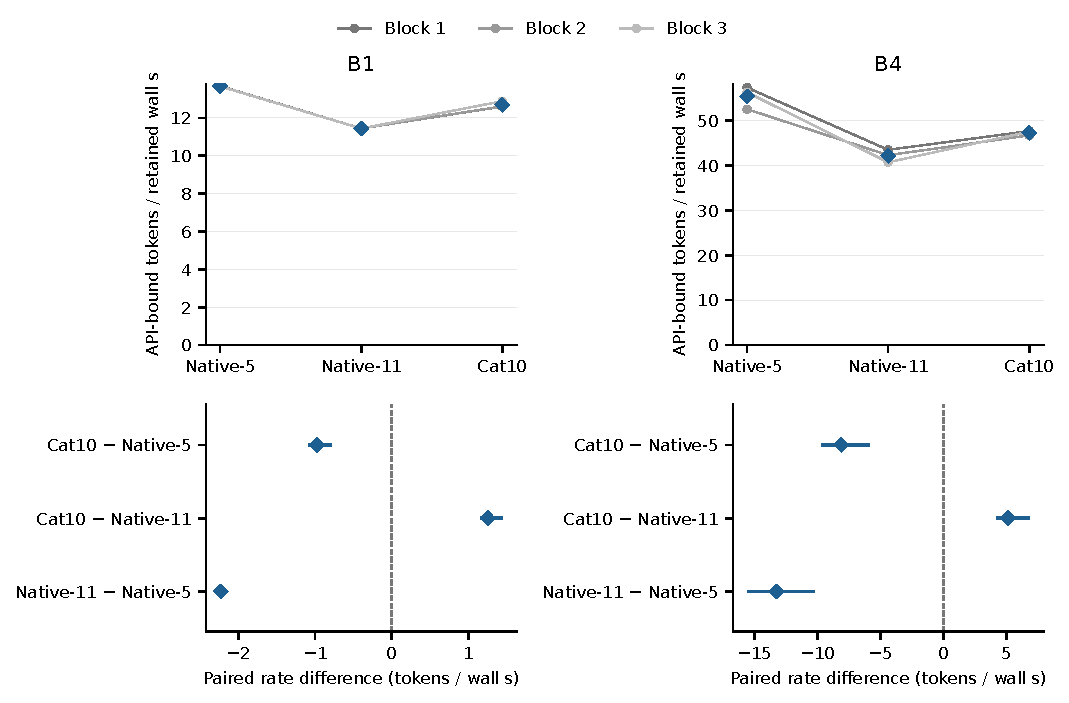
\includegraphics[width=0.94\textwidth]{figures/e1-timing.pdf}
\caption{E1: all eighteen initial fresh-boot cells on the pinned stack. Top: each gray line connects one paired block; blue diamonds mark the mean of three boot rates. Bottom: mean paired differences and the frozen 95\% bootstrap percentile intervals, resampling whole blocks separately at B1 and B4. Rates bind returned API tokens to unique retained wall intervals. These are as-executed instrumented configurations with different attention backends, the disclosed engine-seed deviation, and observed output divergence; they do not isolate a causal tree-algorithm effect.}
\label{fig:e1-timing}
\end{figure*}

\paragraph{Observed continuation divergence}
A retrospective comparison uses the complete timed API-ID streams, not just rate-support tokens. Across the three pairs of arms, three blocks, two batch conditions, and eight prompts, only 14 of 144 same-block prompt-stream pairs are exactly equal. Comparing the three block pairs within each arm/batch gives 72 equal pairs out of 144. Both native B1 arms repeat exactly in all 24 within-arm comparisons apiece; tree B1 does so in 8/24. At B4 the equality counts are 7/24 for MTP-5, 5/24 for MTP-11, and 4/24 for cat10. These dependent pair counts describe the observed streams, not an estimated population failure probability. They neither identify the source of divergence nor establish full-model sequential equivalence. Together with the seed and backend differences, they limit the result to measured output rates of the tested configurations on fixed input prefixes. No matched-continuation, quality-preservation, or isolated algorithm-speedup claim follows. The retrospective diagnostic does not alter the frozen eligibility, rates, intervals, or precision decisions.

\subsection{Single-logits reuse: qualified component comparison}
\label{sec:e8-timing}
E8 isolates the redundant vocabulary projection described in Section~\ref{sec:optimization}. The E1 tree already uses logits reuse. E8 adds a real source-controlled OFF path that recomputes the head for spine selection while retaining the same first-logits candidate extraction. The actual loaded source, rather than an inert environment switch, defines each arm. Cat10 topology, stock \texttt{TREE\_ATTN}, flat-slot KV remapping, model weights, image, B1 occupancy, eager execution, synchronous scheduling, disabled prefix caching, and temperature zero remain fixed. Both engine and API seeds are explicitly 20260921.

Two untimed qualification boots preceded timing. On each of eight frozen prefixes, each arm returned 32 API token IDs. Every qualified proposal evaluated both head paths on the same input: 103 proposals and 515 paired head comparisons per arm passed bitwise whole-logit, argmax, ordered top-two, and packed candidate-tree checks. The gate also checked input/RNG preservation and watched-tensor mutation, with closed recorder and head receipts. Complete API streams reconciled with the emitted ledger, and all eight streams matched across these two qualification boots. These finite checks establish the observed head/candidate invariants; they are not a full-model state-equivalence proof and supply no timing estimate.

The timing campaign then ran three fixed paired blocks in OFF/ON, ON/OFF, and OFF/ON order. Each of the six fresh servers received two 32-token warmups followed by the same eight prefixes at a 128-token budget with EOS enabled. Expensive paired-head checks and captures were disabled; small head-call counters remained in both arms. The final census confirms five vocabulary projections per proposal with reuse ON and ten with reuse OFF. All ten requests in each boot are included in API/ledger reconciliation. The primary rate uses the same retained-decode token/wall support as E1, with at least one eligible interval per timed prefix, all valid slow intervals retained, and no failed-cell replacement or prompt selection. GPU ownership was sampled before, every five seconds during, and after the workload. Every observed GPU process belonged to the single owned container; this does not exclude transient contention between samples.

The prespecified primary statistic is the mean of three paired relative rate differences,
\begin{equation}
 \Delta_{\mathrm{reuse}}=\frac{1}{3}\sum_{b=1}^{3}
 \left(\frac{r_{b,\mathrm{ON}}}{r_{b,\mathrm{OFF}}}-1\right).
\end{equation}
The frozen analysis resamples whole paired blocks 10,000 times with seed 20260921 and reports the 2.5th and 97.5th percentiles. All three complete pairs are required; uncertainty from three blocks is coarse. The ratio of arm means is a secondary diagnostic. The estimator was fixed before any timing data.

\begin{table}[t]
\caption{E8: all three paired B1 blocks. Rates are retained-decode tokens/s for the source-controlled head-reuse comparison. The final ON boot has different continuations and one early EOS; it remains in the primary analysis.}
\label{tab:e8-reuse}
\centering\footnotesize
% Generated only from the complete independently reviewable frozen E8 aggregate.
\begin{tabular}{@{}lrrr@{}}
\toprule
Block & Reuse OFF & Reuse ON & Paired change \\
\midrule
1 & 9.686 & 12.591 & +29.99\% \\
2 & 9.703 & 12.595 & +29.81\% \\
3 & 9.697 & 12.887 & +32.90\% \\
\bottomrule
\end{tabular}

\end{table}

All six initial cells completed with valid sealed evidence. They retained 298--314 intervals each, with at least 29 per prefix and no eligible interval above the 1.5-second diagnostic cutoff. Mean boot rates are 12.691 tokens/s with reuse ON and 9.695 with reuse OFF. The mean paired relative increase is 30.90\%, with a frozen 95\% percentile interval of $[29.81\%,32.90\%]$. Table~\ref{tab:e8-reuse} reports every pair; no run was repeated or replaced. E1 already includes this optimization, so its Cat10 rate must not be multiplied by this relative increase.

Complete timed streams match in 16 of 24 within-pair comparisons and 32 of 48 across-block comparisons within an arm. The third ON boot differs on all eight prefixes; p021 ends at EOS after 101 tokens. Its support remains valid and its outcome is retained. Thus the component contrast reports rates of these as-executed instrumented configurations on fixed prefixes, not equal-output latency or general quality preservation. Same-input head equivalence, reduced head-call count, and cross-boot continuation equality are separate claims. E8 adds B1 attribution evidence for this component; it neither replaces the E1 native/tree comparison nor establishes a fully optimized or composed system gain.

\section{Discussion and Remaining Optimization Evidence}
\label{sec:planned}
The mechanism results constrain the implementation choices. Branch-local recurrence and selected-path publication are separate operations, so a local verifier match cannot establish correct continuation. The fresh incompatible-slot-policy witness also shows why a numerical layout technique must respect the attention backend's address convention. The corrected synchronous flat-map route passes the bounded checks reported above; live convolution/KV byte snapshots, graph execution, cache-hit behavior, stochastic deployment, and full-model sequential equivalence remain outside that coverage.

Sequential replay is a useful reference implementation, but the fresh compact-route comparison does not establish that it is universally more accurate or faster. The local realizations miss frozen numerical, padding, and timing criteria; no compact candidate is promoted. These are implementation-specific findings on the captured operands. They do not establish a defect in the published TreeWY or Bole systems, which were not benchmarked here.

The E1 timing campaign characterizes particular complete configurations. It does not attribute the rate difference to scan, attention, draft construction, acceptance, or replay individually. The tree trails the depth-comparable native chain and exceeds the longer chain under the as-executed settings. Output divergence, different attention backends, and the engine-seed deviation prevent an isolated algorithm-speedup or quality-preservation claim. Retained-decode rate also differs from full-service latency.

E8 supplies a route-specific component comparison for draft-logit reuse, with same-input head checks and measured invocation counts. Its cross-boot continuation divergence still limits the timing claim. Other optimization candidates require compatible active routes, their own numerical and continuation checks, and measurements of each component and its composition on declared support. A fixed-shape or FA2-specific candidate cannot be credited to the current stock-attention caterpillar by combining results across those routes. No such composed optimization gain is claimed in this revision. Appendix~\ref{app:validation} records the remaining validation boundaries.

\section{Conclusion}
\sys{} implements tree verification for a recurrent-hybrid model by connecting an ancestry-aware target forward to accepted-path state publication. A shared descriptor coordinates attention visibility, branch-local GDN computation, convolution history, device probability arithmetic, and the next native continuation. Sequential scan and accepted-path replay make the state lifetime and arithmetic choices explicit; cached state, recomputation, physical layout, and independent-work batching expose the main optimization tradeoffs.

Fresh measurements characterize that implementation rather than all available optimization candidates. The selected synchronous route has bounded numerical, state, and accepted-path evidence. Local compact reconstructions fail the frozen promotion criteria. In eighteen timing boots, the tree averages 12.69 versus native MTP-5's 13.67 tokens/s at batch one, and 47.28 versus 55.38 at batch four, while exceeding MTP-11. Different continuations, backends, and engine seeds constrain those rates to the configurations as executed.

The six-boot single-logits comparison measures a 30.90\% mean paired rate increase over redundant head evaluation at B1, with different continuations in one ON boot. This optimization was already active in the complete-configuration comparison. The resulting contribution is a concrete verifier design, its GPU execution strategy, and scoped component evidence. Further component and composition ablations remain necessary before claiming gains from the unfinished candidates. Broader quality preservation, full-model sequential equivalence, and comparative performance against the authors' external systems remain unestablished.

\appendices
\section{Measurement and Provenance}
\label{app:audit}
\subsection{Sampling provenance remains an explicit limitation}
P0 source reconstruction found repeated target-logit constraints in earlier campaign patchers~\cite{lumo2026levers}. Repeated filtering and differing bonus paths mean that the requested historical sampling settings do not identify a single effective sampler. Historical loaded-extension and model-file identities also remain unresolved; current hashes cannot recover them. We preserve the reconstruction records in the artifact and exclude historical numerical results from this paper. The fresh experiments record their own loaded sources and actual settings, including the E1 engine-seed deviation.

The stored records remain audit evidence, but do not provide a controlled-temperature estimate of the final system's advantage. Likewise, an available correctness test counts as a current passing result only when its execution record establishes the relevant route~\cite{lumo2026archive}.

\subsection{Tokens, events, physical steps, and service time}
Let $a_e$ be accepted drafts and $c_e$ be actual emitted tokens in request verification event $e$. For ordinary nonterminal events, $c_e=a_e+1$ because of a correction/bonus token. End-of-sequence and truncation instead require the actual count. A physical GPU step can contain several request events. A measured decode rate requires output counts and wall intervals from the same event population; component attribution also requires matching the timed operations to those events.

An archived instrument did not supply that matching: its numerator summarizes global request events, whereas its wall intervals retain a pure-decode subset. Its component spans also use different supports. Changing units or substituting a different global token total cannot recover the missing matched observations~\cite{lumo2026archive}. The raw counters, retrospective audit, and reproducible accounting are preserved in the artifact; the derived rate proxies, component chart, and proxy break-even calculation are excluded here. Section~\ref{sec:e1-timing} defines the fresh matched-support measurement. TTFT, TPOT, queueing, cache misses, and full-service throughput remain separate quantities.


The historical quality observations used a selected Astropy subset from SWE-bench Verified~\cite{jimenez2024swe}. They do not provide quality evidence for the fresh fixed-prefix timing campaign; neither chosen subset represents the full benchmark.

\subsection{Four different correctness questions}
\textit{Algebraic correctness} asks whether the recurrence or its reformulation computes the same real-arithmetic function. \textit{Numerical agreement} asks whether particular kernels, layouts, and precisions agree with a selected reference. \textit{Sampler correctness} asks whether the acceptance/residual rule returns its supplied target distribution. \textit{Serving correctness} asks whether these properties survive cache restoration, row reuse, batching, and the next iteration~\cite{yang2024delta,chen2023sampling,lumo2026archive}.

For example, for target probabilities $p$ and proposal probabilities $q$, accepted mass is $\min(p,q)$ under ordinary rejection sampling. Sampling the remaining mass proportional to $(p-q)_+$ gives the target marginal. The argument is conditional on the actual proposal law and target probabilities; substituting stale logits or an incorrect state changes the distribution being sampled~\cite{leviathan2023fast,chen2023sampling}. The same distinction applies to the multidraft reference used here~\cite{miao2023specinfer,lumo2026archive}.

If every iteration supplies the reference conditional probabilities and publishes an equivalent continuation boundary, an induction over emitted tokens gives the reference joint distribution. This is a conditional argument, not a proof that the implemented system satisfies its premises. A tolerance test, zero observed garble, or equal task outcomes does not discharge all those premises.


\section{Validation Scope}
\label{app:validation}
Table~\ref{tab:planned} lists the selected validation scope and deferred extensions. After configuration reconciliation (P0), three core experiments compare arithmetic on identical inputs (E7a), test numerical propagation and accepted-prefix continuation (E2/E7b), and measure the frozen implementation against strong chains (E1). E3 requires compatible route qualification before any candidate can be promoted. E7a has completed kernel measurements, including fresh pilot and confirmation operands. E2/E7b supplies the bounded diagnostic and selected-route evidence above. E1 adds the eighteen-cell as-executed comparison above; its capture pilots and untimed preflights are not additional timing cells. E8 adds the completed six-boot B1 component ablation after two separate qualification boots; these counts do not extend or replace E1.

\begin{table*}[t]
\caption{Selected scope. E7a, bounded E2/E7b checks, eighteen E1 timing cells, and six E8 timing cells are executed, preceded by P0 and their stated qualifications. E3 remains conditional; other entries are deferred.}
\label{tab:planned}
\centering\footnotesize
\begin{tabularx}{\textwidth}{@{}p{0.08\textwidth}p{0.22\textwidth}Y>{\raggedright\arraybackslash}p{0.20\textwidth}@{}}
\toprule
ID & Question & Minimum comparison & Claim enabled \\
\midrule
P0 & What actually ran? & Archived binary, flags, sampling and denominator reconciliation & Correct configuration labels \\
E1 & How does the qualified tree compare with strong chains? & Cat10, depth-comparable chain-5, longer chain-11; actual B1/B4; paired independent boots & As-executed decode-interval rates \\
E7a & Do arithmetic realizations agree? & Same operands: sequential, triangular solve, finite-Neumann; output and commit isolated & Numerical and local-cost characterization \\
E2/E7b & Do errors amplify or corrupt continuation? & Fixed-prefix stage substitutions; layer/final logits; state/KV/conv, sampler and cache fixtures & Scoped continuation and implementation agreement \\
E8 & What does draft-logit reuse change? & Same-input head qualification, then three paired ON/OFF blocks at B1 & Bounded component rate contrast; continuation differences retained \\
E3 & Do optimizations combine? & Conditional scan/accept-walk toggles, individually and together & Composed local speedup \\
E4 & How does memory affect service latency? & Deferred: identical arrival trace and cache-capacity controls & Serving and cache explanation \\
E5 & Is broader task quality preserved? & Deferred: held-out tasks and powered quality design; exact sampler checks stay in E2 & Broader quality evidence \\
E6 & Does the result extend to NVFP4? & Deferred: matched native control and repeated composed tests & Quantization extension \\
E7c & How do authors' systems compare? & Deferred: feasible matched external implementations & Competitive system comparison \\
\bottomrule
\end{tabularx}
\end{table*}

E7a compares local reimplementations of published mechanisms, not the authors' systems. Identical captured operands and chosen paths isolate solver error from commit error. High-precision recurrence and each pinned native GPU path serve distinct reference roles. Its fresh synthetic stress test, the verified eight-prefix pilot, and the 32-prefix confirmation set evaluated against the record frozen from that pilot are reported in Section~\ref{sec:e7a-pilot}, including all identified frozen-rule failures and the retrospective audit of omitted checks. Those sample counts belong to E7a. Neither compact candidate met the frozen local criteria, so neither is promoted to an integrated serving or performance claim. E7b instead reports the bounded, single-prefix verifier-only and commit-only diagnostics and the offline fixed-input continuation in Section~\ref{sec:e7b-diagnostic}. The matched input-aligned windows are observed controls, not a general forced-path facility: the served route refuses the older forced-spine diagnostic. No combined-candidate confirmation campaign or powered task-quality study has been completed. Broader promotion would require those separate verification, commitment, combined-route, and continuation checks; the present failures remain reportable numerical findings.

E1 supplies controlled-prefix replay evidence for the tested instrumented configurations (Section~\ref{sec:e1-timing}). Its fixed-input prefixes produce different continuations, and the engine-seed mismatch prevents a fully controlled-settings interpretation. Matching numerator and denominator support fixes an accounting problem; it does not establish equivalent outputs, quality, or full-service latency. All eighteen initial cells are retained, and all six contrasts meet the prespecified precision target under coarse three-block resampling. Compact-route performance remains deferred because its numerical promotion criteria failed.

E8 isolates the redundant head invocation on the selected B1 route (Section~\ref{sec:e8-timing}). All six timing boots and all three paired blocks are retained. Qualification and clean-mode invocation counts support the component interpretation, while the final ON boot's divergent continuations limit it to as-executed rates. No B4, quality-preservation, or composed optimization claim follows.

E2 combines existing analytic multidraft identities, multistep sampling tests, biased-selector controls, and accepted-path state fixtures~\cite{lumo2026archive} with the source-bound and actual-route checks in Section~\ref{sec:selected-route}. Graph execution, prefix-cache hits, stochastic deployment, and a full-model sequential oracle remain outside this finite qualification. Source availability alone is not a passing execution record, and historical numerical or garble checks do not prove distribution preservation.

\label{ReferencesStart}
\bibliographystyle{IEEEtran}
\bibliography{ref}
\end{document}
